\chapter{Capa Límite}
	
	\begin{itemize}
		\item Por muy baja que sea la viscosidad de un fluido, en contacto con un
		sólido, la velocidad es la del sólido (generalmente, cero).
		\item Esto implica una zona de aumento progresivo de la velocidad desde
		0 hasta la velocidad del flujo en zonas no influenciadas por el sólido,
		$U_{\infty}$.
		\item Esta zona se denomina \textcolor{red}{\href{https://en.wikipedia.org/wiki/Boundary_layer}{capa límite}},
		y en ella se producen los efectos que realmente actúan sobre el sólido
		(arrastre, \ldots ).
		\item La capa límite puede ser laminar o turbulenta. El \textcolor{blue}{número
			de Reynolds local} que controla el régimen se define como 
		\[
		\text{Re}_{x}=\frac{\rho U_{\infty}x}{\mu}=\frac{U_{\infty}x}{\nu},
		\]
		donde $\rho$ es la densidad del fluido, $\mu$ es la viscosidad
		dinámica, $\nu$ es la viscosidad cinemática y $x$ es la distancia
		desde el punto en el que el flujo entra en contacto con el sólido.
		No hay un número concreto para la transición a capa límite turbulenta,
		pero está alrededor de $10^{6}$.
	\end{itemize}

	Consideremos, como ejemplo, el flujo sobre y bajo una placa lisa.

\begin{center}
	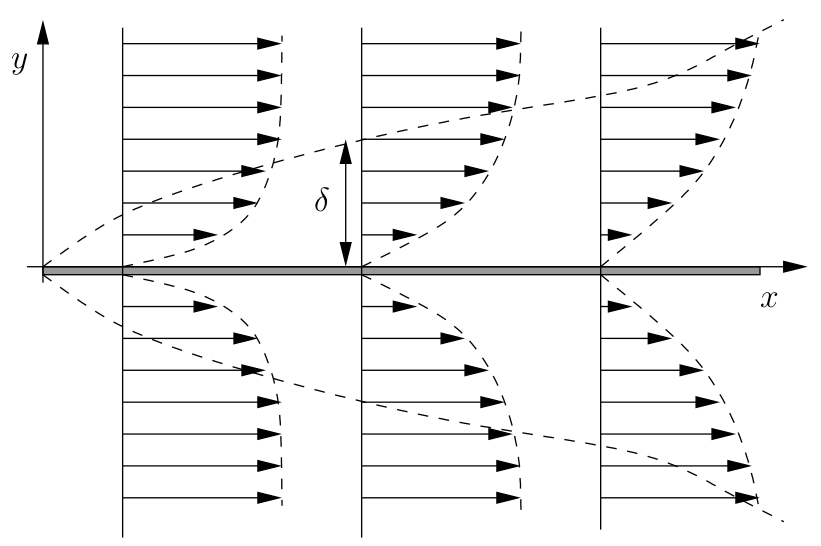
\includegraphics[width=0.7\linewidth]{TeX_files/chapter08-CapaLimite/capa1}
\end{center}
	
	
	El \textcolor{red}{espesor $\delta$} de la capa límite se define
	como la distancia de la placa para la cual la velocidad $v$ del flujo
	alcanza el 99\% de $U_{\infty}$.
	
	Pero se definen \href{https://en.wikipedia.org/wiki/Boundary_layer_thickness}{otros espesores}
	de la capa límite:
	
	\begin{itemize}
		\item \textcolor{red}{espesor de desplazamiento $\delta^{*}$}. Debido a
		la disminución de velocidad en la proximidad del sólido, se produce
		una pérdida de caudal. Se define $\delta^{*}$ como la distancia que
		habría que desplazar la placa con un fluido ideal sin viscosidad (no
		hay, por tanto, la condición de no deslizamiento) para que la pérdida
		de caudal fuese la misma.
		
		\begin{tabular}{cc}
			\begin{minipage}[c]{0.4\textwidth}%
\begin{center}
	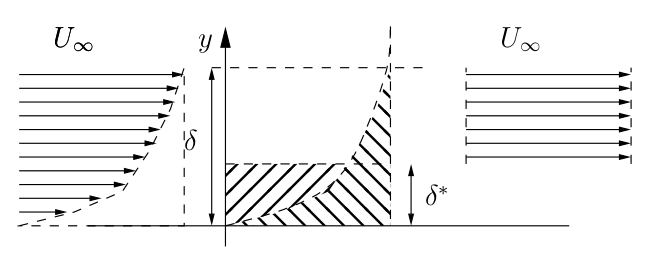
\includegraphics[width=\linewidth]{TeX_files/chapter08-CapaLimite/capa2}
\end{center}

			\end{minipage} & %
			\begin{minipage}[c]{0.5\textwidth}%
				
				\[
				U_{\infty}\delta^{*}b=\int_{0}^{\delta}\left(U_{\infty}-u\right)b\dif y
				\]
				
				
				\begin{equation}
					\Rightarrow\boxed{\delta^{*}=\int_{0}^{\delta}\left(1-\frac{u}{U_{\infty}}\right)\dif y}
				\end{equation}
				
				%
			\end{minipage}\tabularnewline
		\end{tabular}

		\item \textcolor{red}{espesor de cantidad de movimiento $\theta$}. Es la
		misma idea, pero con pérdida de cantidad de movimiento, en lugar de
		caudal. 
		\[
		U_{\infty}^{2}\theta=\int_{0}^{\delta}u\left(U_{\infty}-u\right)\dif y
		\]
		
		\begin{equation}
			\Rightarrow\boxed{\theta=\int_{0}^{\delta}\frac{u}{U_{\infty}}\left(1-\frac{u}{U_{\infty}}\right)\dif y}
		\end{equation}
		
		
	\end{itemize}
	Sobre cada pared de la placa se realiza un esfuerzo $\tau_{p}$, dado
	por 
	\[
	\tau_{p}=\mu\left.\dparc{u}{y}\right|_{y=0}
	\]
	
	El \textcolor{red}{coeficiente de esfuerzo superficial de pared} se
	define como 
	
\begin{equation}
		C_{f}=\frac{\tau_{p}}{\frac{1}{2}\rho U_{\infty}^{2}}
\end{equation}
	
	


\section{Capa límite laminar. Ecuación de Blasius}

	
	Considerando flujo estacionario, sin gradiente de presión, y que $\dparc{u}{y}\gg\dparc{u}{x}$,
	las ecuaciones de continuidad y NS son 
	\begin{eqnarray}
		u\dparc{u}{x}+v\dparc{u}{y}=\nu\dparcsec{u}{y}\\
		\dparc{u}{x}+\dparc{v}{y}=0
	\end{eqnarray}
	con las condiciones de contorno 
	\begin{eqnarray*}
		y=0\, & \rightarrow & \,u=0\\
		y=\infty\, & \rightarrow & \,\left\{ \begin{matrix}u=U_{\infty}\\
			\deriv{u}{y}=0
		\end{matrix}\right.
	\end{eqnarray*}
	
	Estas son conocidas como \textit{Ecuaciones de Prandtl}.
	

	
	Dado que el flujo es bidimensional, podemos usar la función de corriente
	$\psi$, 
	\begin{eqnarray*}
		u & = & \dparc{\psi}{y}\\
		v & = & -\dparc{\psi}{x}
	\end{eqnarray*}
	de esta forma, la ecuación de continuidad de cumple de forma automática.
	La ecuación de NS queda entonces como 
	\[
	\dparc{\psi}{y}\,\frac{\partial^{2}\psi}{\partial x\partial y}-\dparc{\psi}{x}\,\dparcsec{\psi}{y}=\nu\frac{\partial^{3}\psi}{\partial y^{3}}
	\]
	

	
	Para poder tratar esta ecuación se definen las variables adimensionales
	$f$ y $\eta$, con $\eta=\sqrt{\frac{U_{\infty}}{\nu x}}\,y$ y $f$
	es tal que $\deriv{f}{\eta}=\frac{u}{U_{\infty}}=\frac{1}{U_{\infty}}\dparc{\psi}{y}$.
	
	Al substituir en la ecuación de NS y tras varias operaciones algebraicas,
	obtenemos 
	\[
	\boxed{2\frac{\dif^{3}f}{\dif\eta^{3}}+f\derivsec{f}{\eta}=0}
	\]
	con las condiciones de contorno
	\[
	\begin{cases}
		\eta=0 & \rightarrow\,f=\deriv{f}{\eta}=0\\
		\eta=\infty & \rightarrow\,\deriv{f}{\eta}=1
	\end{cases}
	\]
	
	Esta es la conocida como \textcolor{red}{\href{https://en.wikipedia.org/wiki/Blasius_boundary_layer}{ecuación de Blasius}}
	(1908), y no se puede resolver analíticamente.

	
	La resolución numérica de esta ecuación indica que el espesor de la
	capa límite se alcanza para $\eta\approx5.0$. Es decir, 
	\[
	\delta\approx\frac{5.0}{\sqrt{\frac{U_{\infty}}{\nu x}}}=\frac{5.0x}{\sqrt{\text{Re}_{x}}}.
	\]
	Los otros espesores son, calculados mediante integración numérica,
	\begin{eqnarray*}
		\delta^{*} & = & 0.344\,\delta\\
		\theta & = & 0.133\,\delta
	\end{eqnarray*}
	
	El esfuerzo superficial sobre la placa viene dado por 
	\[
	\tau_{p}=\mu\left.\dparc{u}{y}\right|_{y=0}=\mu U_{\infty}\sqrt{\frac{U_{\infty}}{\nu x}}\,\left.\derivsec{f}{\eta}\right|_{\eta=0}
	\]
	

	
	De la misma solución numérica de la ecuación de Blasius, se comprueba
	que 
	\[
	\tau_{p}=0.332U_{\infty}\sqrt{\frac{\rho\mu U_{\infty}}{x}}=\frac{0.332\rho U_{\infty}^{2}}{\sqrt{\text{Re}_{x}}}
	\]
	y el coeficiente de esfuerzo superficial es 
	\[
	C_{f}=\frac{0.664}{\sqrt{\text{Re}_{x}}}
	\]
	
	Podemos calcular la fuerza de arrastre sobre una placa de longitud
	$L$ y amplitud $b$, 
	\[
	F_{D}=b\int_{0}^{L}\tau_{p}\dif x=0.332\rho U_{\infty}^{2}b\int_{0}^{L}\frac{1}{\sqrt{\text{Re}_{x}}}\dif x=0.664b\sqrt{\rho\mu LU_{\infty}^{3}}
	\]
	
	El \textcolor{red}{coeficiente de arrastre} sobre la placa será 
	\[
	C_{D}=\frac{F_{D}}{\frac{1}{2}\rho U_{\infty}^{2}bL}=\frac{1.328}{\sqrt{\text{Re}_{L}}}
	\]
	


\section[Ecuación de von Kármán]{Ecuación integral de von Kármán}

	
	\begin{tabular}{cc}
		\begin{minipage}[c]{0.4\textwidth}%
			\begin{center}
				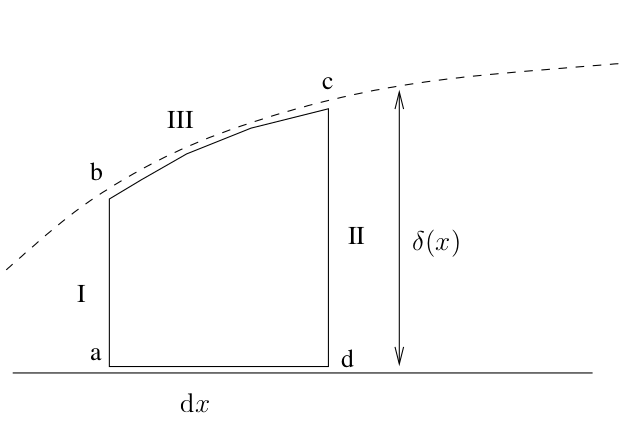
\includegraphics[width=1\linewidth]{TeX_files/chapter08-CapaLimite/vonKarman}
			\end{center}
			
		\end{minipage} & %
		\begin{minipage}[c]{0.5\textwidth}%
			Continuidad: 
			\begin{eqnarray*}
				\text{I :}Q_{ab} & = & -\int_{0}^{\delta}u(y)b\dif y\\
				\text{II :}Q_{cd} & = & -\left[Q_{ab}+\dparc{Q_{ab}}{x}\dif x\right]
			\end{eqnarray*}
			
			De aqui obtenemos el caudal que entra por III: 
			\[
			Q_{bc}=-b\dparc{}{x}\left[\int_{0}^{\delta}u(y)\dif y\right]\dif x
			\]
			%
		\end{minipage}\tabularnewline
	\end{tabular}

	
	Por otro lado, aplicamos la conservación de la cantidad de movimiento,
	\[
	F_{S}=\int_{SC}\rho u\vec{u}\cdot\dif\vec{S}
	\]
	
	\begin{eqnarray*}
		\text{I :} & -b\int_{0}^{\delta}\rho u(y)^{2}\dif y\\
		\text{II :} & b\left[\int_{0}^{\delta}\rho u(y)^{2}\dif y+\dparc{}{x}\left(\int_{0}^{\delta}\rho u(y)^{2}\dif y\right)\dif x\right]\\
		\text{III :} & -U_{\infty}b\dparc{}{x}\left[\int_{0}^{\delta}\rho u(y)\dif y\right]\dif x
	\end{eqnarray*}
	
	\[
	F_{S}=\left[-\deriv{p}{x}\,\dif x\delta-\tau_{p}\dif x\right]\,b
	\]
	
	\[
	-\deriv{p}{x}\delta-\tau_{p}=\dparc{}{x}\left(\int_{0}^{\delta}\rho u(y)^{2}\dif y\right)-U_{\infty}\dparc{}{x}\int_{0}^{\delta}\rho u(y)\dif y
	\]
	
	
	El gradiente de presiones se obtiene haciendo Bernoulli por la parte
	exterior de la capa límite, 
	\[
	\deriv{p}{x}=-\rho U_{\infty}\deriv{U_{\infty}}{x}
	\]
	y, operando, llegamos a 
	\[
	\boxed{\tau_{p}=\rho\deriv{}{x}\left(U_{\infty}^{2}\theta\right)+\rho\delta^{*}U_{\infty}\deriv{U_{\infty}}{x}}
	\]
	
	Esta es la \textcolor{red}{ecuación integral de cantidad de movimiento},
	y es una ecuación diferencial ordinaria, que nos permite calcular
	$\delta$ a partir de una suposición sobre la forma del perfil de
	velocidades.
	
	Si \textcolor{blue}{no hay gradiente de presiones}, $\deriv{U_{\infty}}{x}=0$,
	y la ecuación se reduce a
	
	\[
	\tau_{p}=\rho\deriv{}{x}\left(U_{\infty}^{2}\theta\right)
	\]
	
	
	\subsection*{Ejemplo:}
		Supongamos que el perfil de velocidades es de forma parabólica, 
		\[
		u=a+by+cy^{2}
		\]
		Las condiciones de contorno son, para $y=0$, $u=0$, y para $y=\delta$,
		$u=U_{\infty}$ y $\deriv{u}{y}=0$. Esto lleva a 
		\[
		\frac{u}{U_{\infty}}=2\zeta-\zeta^{2}
		\]
		con $\zeta=\frac{y}{\delta}$. El esfuerzo tangencial sobre la pared,
		según este perfil, es 
		\[
		\tau_{p}=\mu\left.\dparc{u}{y}\right|_{y=0}=2\frac{U_{\infty}\mu}{\delta}
		\]
		
		El espesor de cantidad de movimiento es {\small{}
			\[
			\theta=\int_{0}^{\delta}\frac{u(y)}{U_{\infty}}\left(1-\frac{u(y)}{U_{\infty}}\right)\dif y=\delta\int_{0}^{1}\frac{u(\zeta)}{U_{\infty}}\left(1-\frac{u(\zeta)}{U_{\infty}}\right)\dif\zeta=\frac{2}{15}\delta
			\]
		}Substituyendo en la ecuación integral de cantidad de movimiento sin
		gradiente de presiones, obtenemos 
		\[
		2\frac{U_{\infty}\mu}{\delta}=\frac{2}{15}\rho U_{\infty}^{2}\deriv{\delta}{x}
		\]
		que nos lleva a 
		\[
		\frac{1}{2}\delta^{2}=\frac{15\mu}{\rho U_{\infty}}x+C
		\]
		
		Dado que, para $x=0$, el inicio de la placa, la capa límite ha de
		tener un espesor nulo, $C=0$, de forma que 
		\[
		\delta=\sqrt{\frac{30\mu x}{\rho U_{\infty}}}=\frac{5.48x}{\sqrt{\text{Re}_{x}}}
		\]
		El esfuerzo tangencial en la pared es, para el perfil parabólico,
		\[
		\tau_{p}=\frac{0.365\rho U_{\infty}^{2}}{\sqrt{\text{Re}_{x}}},
		\]
		y los coeficientes de fricción y arrastre son 
		\[
		C_{f}=\frac{0.730}{\sqrt{\text{Re}_{x}}},\;C_{D}=\frac{1.460}{\sqrt{\text{Re}_{L}}}
		\]

	
	\subsection*{Actividad 1:}
		Repetir todos los pasos del ejemplo con un perfil sinusoidal, 
		\[
		\frac{u}{U_{\infty}}=\sin\left(\frac{\pi}{2}\zeta\right)
		\]

	
	
	\begin{tabular}{cc}
		\begin{minipage}[c]{0.75\textwidth}%
			Esta gráfica muestra la comparación entre el perfil de Blasius y los perficles parabólico y sinusiodal.
			\begin{center}
				\includegraphics[width=1\linewidth]{../../MFGA/Presentaciones/19-capalimite1/perfiles}
			\end{center}
			
			\begin{flushleft}
				\par\end{flushleft}%
		\end{minipage} & %
		\begin{minipage}[c]{0.25\textwidth}% 
			Estos son los valores numéricos para el perfil de Blasius.
				\begin{center}
					\begin{tabular}{|c|c|}
						\hline 
						$y/\delta$  & $u/U_{\infty}$ \tabularnewline
						\hline 
						\hline 
						0.0  & 0.0 \tabularnewline
						\hline 
						0.04  & 0.06641 \tabularnewline
						\hline 
						0.08  & 0.13277 \tabularnewline
						\hline 
						0.12  & 0.19894 \tabularnewline
						\hline 
						0.16  & 0.26471 \tabularnewline
						\hline 
						0.2  & 0.32979 \tabularnewline
						\hline 
						0.24  & 0.39378 \tabularnewline
						\hline 
						0.28  & 0.45627 \tabularnewline
						\hline 
						0.32  & 0.51676 \tabularnewline
						\hline 
						0.36  & 0.57477 \tabularnewline
						\hline 
						0.4  & 0.62977 \tabularnewline
						\hline 
						0.44  & 0.68132 \tabularnewline
						\hline 
						0.48  & 0.72899 \tabularnewline
						\hline 
						0.52  & 0.77246 \tabularnewline
						\hline 
						0.56  & 0.81152 \tabularnewline
						\hline 
						0.6  & 0.84605 \tabularnewline
						\hline 
						0.64  & 0.87609 \tabularnewline
						\hline 
						0.68  & 0.90177 \tabularnewline
						\hline 
						0.72  & 0.92333 \tabularnewline
						\hline 
						0.76  & 0.94112 \tabularnewline
						\hline 
						0.8  & 0.95552 \tabularnewline
						\hline 
						0.84  & 0.96696 \tabularnewline
						\hline 
						0.88  & 0.97587 \tabularnewline
						\hline 
						0.92  & 0.98269 \tabularnewline
						\hline 
						0.96  & 0.98779 \tabularnewline
						\hline 
						1  & 0.99155 \tabularnewline
						\hline 
					\end{tabular}
					\par\end{center}
		\end{minipage}\tabularnewline
	\end{tabular}

\section{Capa límite turbulenta}

	
	Partimos de la ecuación integral de cantidad de movimiento, que es
	válida tanto para flujo laminar como para turbulento. Consideremos
	que no hay gradiente de presiones. 
	\[
	\tau_{p}=\rho U_{\infty}^{2}\deriv{\theta}{x}
	\]
	
	Esta ecuación se puede escribir en términos adimensionales 
	\[
	C_{f}=2\deriv{\theta}{x}
	\]
	
	Como vimos en el tema de Turbulencia, el perfil turbulento de velocidades
	cerca de la pared se puede escribir como una ley logarítmica 
	\[
	\frac{u}{u^{*}}=\frac{1}{\kappa}\ln\frac{\rho u^{*}y}{\mu}+B\qquad;\qquad u^{*}=\sqrt{\frac{\tau_{p}}{\rho}}\quad\text{(velocidad de fricción)}
	\]
	

	
	Esta velocidad de fricción también se puede escribir como 
	\[
	u^{*}=\sqrt{\frac{1}{2}C_{f}U_{\infty}^{2}}=U_{\infty}\sqrt{\frac{C_{f}}{2}}
	\]
	
	Para $y=\delta$, la velocidad de fricción debe cumplir la ley logarítmica
	\[
	\frac{U_{\infty}}{u^{*}}=\frac{1}{\kappa}\ln\frac{\rho u^{*}\delta}{\mu}+B
	\]
	
	\[
	\sqrt{\frac{2}{C_{f}}}=\frac{1}{\kappa}\ln\left[\frac{\delta}{\nu}U_{\infty}\sqrt{\frac{C_{f}}{2}}\right]+B=\frac{1}{\kappa}\ln\left[\text{Re}_{\delta}\sqrt{\frac{C_{f}}{2}}\right]+B
	\]
	
	Debería ser posible resolver esta ecuación para obtener $C_{f}$ en
	función de $\text{Re}_{\delta}$, pero es imposible hacerlo de forma
	explícita, y usamos una forma aproximada 
	\[
	C_{f}=\frac{0.02}{\text{Re}_{\delta}^{1/6}}
	\]
	

	
	Introduciendo esta expresión en la ecuación integral de cantidad de
	movimiento, obtenemos 
	\[
	\frac{0.02}{\text{Re}_{\delta}^{1/6}}=2\deriv{\theta}{x}
	\]
	
	Con una expresión para el perfil de velocidades, podemos calcular
	\[
	\theta=\delta\int_{0}^{1}\frac{u(\zeta)}{U_{\infty}}\left(1-\frac{u(\zeta)}{U_{\infty}}\right)\dif\zeta
	\]
	con $\zeta=y/\delta$. 
	
	La expresión podria ser la ley logarítmica, pero complicaría de nuevo
	enormemente el cálculo, de forma que se usa una ley aproximada de
	potencia, $\frac{u(\zeta)}{U_{\infty}}=\zeta^{1/7},$ y se obtiene
	\[
	\theta=\delta\int_{0}^{1}\zeta^{1/7}\left(1-\zeta^{1/7}\right)\dif\zeta=\frac{7}{72}\delta.
	\]
	

	
	La ecuación integral de cantidad de movimiento queda entonces 
	\[
	\frac{0.02}{\text{Re}_{\delta}^{1/6}}=\frac{7}{36}\deriv{\delta}{x}
	\]
	
	\[
	\Rightarrow\,\text{Re}_{\delta}^{-1/6}=9.72\deriv{\delta}{x}=9.72\deriv{\text{Re}_{\delta}}{\text{Re}_{x}}
	\]
	
	\[
	\Rightarrow\text{Re}_{\delta}=0.16\text{Re}_{x}^{6/7}\,\Rightarrow\,\boxed{\delta=\frac{0.16x}{\text{Re}_{x}^{1/7}}}
	\]
	y de aqui es posible obtener también $C_{f}$, 
	\[
	C_{f}=0.02\text{Re}_{\delta}^{-1/6}=\frac{0.027}{\text{Re}_{x}^{1/7}}
	\]
	

	
	\subsection*{Ejemplo:}
		Consideremos agua con  sobre una placa plana rugosa, de forma que
		se induce una capa lí mite turbulenta desde el principio de la placa.
		Queremos calcular los espesores ,  y  y el esfuerzo superficial para
		. Compararemos con los resultados si la placa fuese completamente
		lisa.Calculamos en primer lugar el número de Reynolds local, $\text{Re}_{x}=\frac{U_{\infty}x}{\nu}=\frac{1\times1}{10^{-6}}=10^{6},$
		de forma que los espesores son 
		\begin{eqnarray*}
			\delta & = & \frac{0.16x}{\text{Re}_{x}^{1/7}}=\frac{0.16\times1}{10^{6/7}}=0.022\,\text{m}\\
			\delta^{*} & = & \delta\int_{0}^{1}\left(1-\zeta^{1/7}\right)\dif\zeta=\frac{1}{8}\delta=0.0028\,\text{m}\\
			\theta & = & \delta\int_{0}^{1}\zeta^{1/7}\left(1-\zeta^{1/7}\right)\dif\zeta=\frac{7}{72}\delta=0.0022\,\text{m}
		\end{eqnarray*}

		y el esfuerzo superficial es {\small{}
			\[
			\tau_{p}=C_{f}\frac{1}{2}\rho U_{\infty}^{2}=\frac{0.027}{\text{Re}_{x}^{1/7}}\frac{1}{2}\rho U_{\infty}^{2}=\frac{0.027}{10^{6/7}}\times\frac{1}{2}\times{1000}\times{1}=1.88\,\text{N}/\text{m}^{2}
			\]
		}
		
		Los cálculos de los espesores para una placa completamente lisa,
		y, por tanto, capa límite laminar, dan {\small{}
			\begin{eqnarray*}
				\delta & = & \frac{5.0x}{\sqrt{\text{Re}_{x}}}=\frac{5.0\times1}{\sqrt{10^{6}}}=0.005\,\text{m}=5\,\text{mm}\\
				\delta^{*} & = & 0.344\,\delta=0.0017\,\text{m}=1.7\,\text{mm}\\
				\theta & = & 0.133\,\delta=0.00066\,\text{m}=0.66\,\text{mm}
			\end{eqnarray*}
		} es decir, unas 4 veces más pequeños.
		
		El esfuerzo superficial es {\small{}
			\[
			\tau_{p}=C_{f}\frac{1}{2}\rho U_{\infty}^{2}=\frac{0.664}{\sqrt{\text{Re}_{x}}}\frac{1}{2}\rho U_{\infty}^{2}=\frac{0.664}{\sqrt{10^{6}}}\frac{1}{2}\times1000\times1=0.332\,\text{N}/\text{m}^{2},
			\]
		} unas 6 veces más pequeño que en el caso de placa rugosa.

		Supongamos que la placa hace un metro de ancho. La fuerza que hace
		el flujo de agua sobre una cara, hasta $L=1\,\text{m}$, es 
			\[
			F_{D}=\int_{S}\tau_{p}\dif S=b\int_{0}^{L}C_{f}\frac{1}{2}\rho U_{\infty}^{2}\dif x=b\frac{1}{2}\rho U_{\infty}^{2}\int_{0}^{L}C_{f}\dif x=C_{D}\frac{1}{2}\rho U_{\infty}^{2}bL
			\]
		
		
		En el caso turbulento,
			\[
			F_{D}=b\frac{1}{2}\rho U_{\infty}^{2}\int_{0}^{L}\frac{0.027}{\re_{x}^{1/7}}\dif x=\frac{1}{2}\rho U_{\infty}^{2}bL\frac{0.031}{\re_{L}^{1/7}}=\frac{1}{2}\times1000\times1\times1\times\frac{0.031}{{10^{6}}^{1/7}}=2.15\,\text{N}
			\]
		
		
		En el caso laminar,
			\[
			F_{D}=b\frac{1}{2}\rho U_{\infty}^{2}\int_{0}^{L}\frac{0.664}{\re_{x}^{1/2}}\dif x=\frac{1}{2}\rho U_{\infty}^{2}bL\frac{1.328}{\re_{L}^{1/2}}=\frac{1}{2}\times1000\times1\times1\times\frac{1.328}{{10^{6}}^{1/2}}=0.664\,\text{N}
			\]
		

\section{Capa límite con gradiente de presiones. Separación de flujo}

	
	¿ Qué ocurre cuando hay gradiente de presiones, o, lo que es lo mismo,
	$\deriv{U_{\infty}}{x}\neq0$ ?
	\begin{itemize}
		\item Si {\small{}
			\[
			\deriv{U_{\infty}}{x}>0\,\Rightarrow\,\deriv{p}{x}<0
			\]
		} se dice que tenemos un \textcolor{red}{gradiente de presiones favorable},
		y no ocurre nada especial. Solo que la ecuación integral de cantidad
		de movimiento es más complicada.
		\item Pero si {\small{}
			\[
			\deriv{U_{\infty}}{x}<0\,\Rightarrow\,\deriv{p}{x}>0
			\]
		} hay un \textcolor{red}{gradiente de presiones adverso} y es posible
		que ocurra una \textcolor{red}{\href{https://en.wikipedia.org/wiki/Flow_separation}{separación de flujo}}.
	\end{itemize}
	Ésto último ocurre cuando la capa lí mite crece tanto que no sólo
	el flujo en la pared es nulo, sino también su derivada {\small{}
		\[
		\left.\deriv{u}{y}\right|_{y=0}=0\,\Rightarrow\,\tau_{p}=0.
		\]
	}{\small\par}

	
\begin{center}
	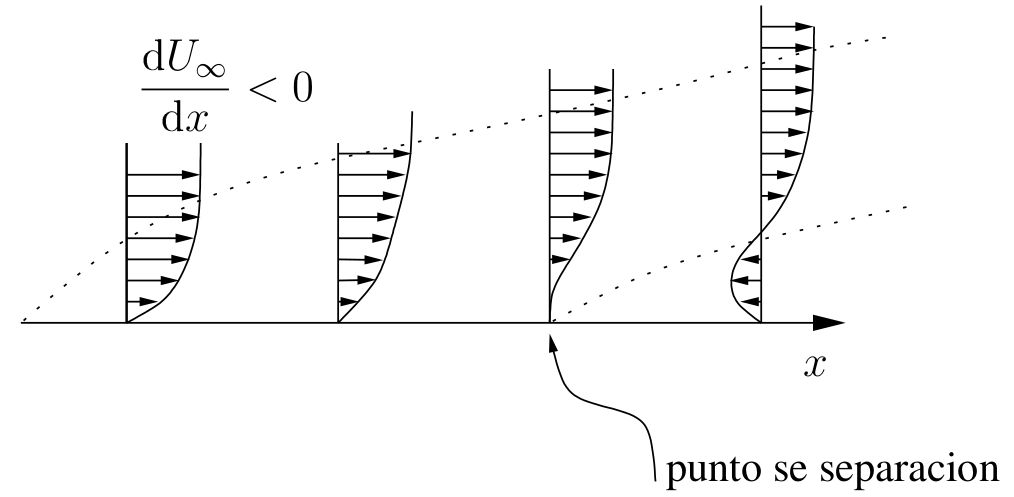
\includegraphics[width=0.7\linewidth]{TeX_files/chapter08-CapaLimite/sepa}
\end{center}


	
	Recordemos que las expresiones para $C_{f}=\frac{\tau_{p}}{\frac{1}{2}\rho U_{\infty}^{2}}$
	son 
	\[
	C_{f}=\frac{\text{cte}}{\sqrt{\re_{x}}}\qquad\text{para flujo laminar}
	\]
	\[
	C_{f}=\frac{\text{cte}}{\re_{x}^{1/7}}\qquad\text{para flujo turbulento}
	\]
	lo cual implica que $\tau_{p}$ se anula únicamente para $\re_{x}\rightarrow\infty$.
	Sin embargo, estas expresiones fueron deducidas para el caso de gradiente
	de presiones nulo.
	
	La ecuación integral de cantidad de movimiento es 
	\[
	\tau_{p}=\rho\deriv{}{x}\left(U_{\infty}^{2}\theta\right)+\rho\delta^{*}U_{\infty}\deriv{U_{\infty}}{x}
	\]
	
	Desarrollándola y con la definición de $C_{f}$ podemos deducir 
	\[
	\frac{C_{f}}{2}=\deriv{\theta}{x}+(H+2)\frac{\theta}{U_{\infty}}\deriv{U_{\infty}}{x}\quad\text{; con}\,H=\frac{\delta^{*}}{\theta}\quad\textbf{factor de forma}
	\]
	
	
	Si calculamos $U_{\infty}(x)$, podemos integrar esta ecuación si
	conocemos $H(\theta)$ y $C_{f}(\theta)$ para encontrar el punto
	$x$ en el que ocurre la separación de flujo ($C_{f}=0$).\medskip{}
	


			Para flujo turbulento el cálculo es demasiado complicado y se deja
			fuera de este curso. Pero es importante notar que el hecho de que
			en la capa límite turbulenta $\theta$ sea mucho menor (en relación
			a $\delta$) que en la laminar hace que separarla de la superficie
			sólida sea más dificil. %

Esta gráfica muestra la comparación, para el mismo espesor, del perfil laminar (Blasius) y turbulento.

\begin{center}
	\includegraphics[width=0.7\linewidth]{../../MFGA/Presentaciones/20-capalimite2/perfiles}
\end{center}


\subsection{El método de Thwaites}
	
	Para capa límite laminar, en 1949 Thwaites encontró de forma experimental
	la relación 
	\[
	S(\lambda)=(\lambda+0.09)^{(0.62)},
	\]
	donde $S=\frac{\tau_{p}\theta}{\mu U_{\infty}}=\frac{1}{2}C_{f}\re_{\theta}$
	es un esfuerzo superficial adimensional, y $\lambda=\frac{\theta^{2}}{\nu}\deriv{U_{\infty}}{x}$
	es un espesor de cantidad de movimiento adimensional. Es necesario
	conocer el valor de $\theta$, que se puede calcular con la expresión
	también de Thwaites 
	\[
	\theta^{2}(x)=\theta_{0}^{2}\left(\frac{U_{0}}{U_{\infty}(x)}\right)^{6}+\frac{0.45\nu}{U_{\infty}^{6}(x)}\int_{0}^{x}U_{\infty}^{5}(x)\dif x
	\]
	
	Con esta expresión es posible calcular $\tau_{p}$ con gradiente de
	presiones y el punto $x$ en el que se produce la separación ($\lambda=-0.09$)
	con un error relativamente pequeño ($\pm10\%)$ respecto a la resolución
	numérica de las ecuaciones de capa límite.

	
	\subsection*{Ejemplo:}
		Consideremos una ley lineal de velocidad 
		\[
		U_{\infty}=U_{0}\left(1-\frac{x}{L}\right).
		\]
		
		Dado que la velocidad $U_{\infty}$ decrece con $x$, la presión crece,
		y tendremos un gradiente de presiones adverso. Si nos aseguramos de
		que en todo momento el flujo es laminar, podemos usar el método de
		Thwaites para calcular el punto de separación del flujo.
		
		Suponiendo que $\theta_{0}=0$, el espesor de cantidad de movimiento
		de la capa lí mite es {\footnotesize{}
			\[
			\theta^{2}(x)=\frac{0.45\nu}{U_{\infty}^{6}(x)}\int_{0}^{x}U_{\infty}^{5}(x)\dif x=\frac{0.45\nu}{U_{0}^{6}}\left(1-\frac{x}{L}\right)^{-6}\int_{0}^{x}U_{0}^{5}\left(1-\frac{x}{L}\right)^{5}\dif x
			\]
		} 
		\[
		\theta^{2}(x)=0.075\frac{\nu L}{U_{0}}\left[\left(1-\frac{x}{L}\right)^{-6}-1\right]
		\]
		
		y $\lambda$ es entonces 
		\[
		\lambda=\frac{\theta^{2}}{\nu}\deriv{U_{\infty}}{x}=-\frac{\theta^{2}U_{0}}{\nu L}=-0.075\left[\left(1-\frac{x}{L}\right)^{-6}-1\right]
		\]
		
		La separación del flujo se da para $\lambda_{sep}=-0.09$, es decir,
		\[
		\lambda_{sep}=-0.09=-0.075\left[\left(1-\frac{x_{sep}}{L}\right)^{-6}-1\right]
		\]
		
		\[
		\Rightarrow\,\frac{x_{sep}}{L}=0.123
		\]
		
		La solución exacta obtenida mediante simulación numérica es $x_{sep}=0.120L$.

	
	Para calcular $C_{f}$ en cualquier punto $\frac{x}{L}$ \textbf{antes}
	de la separación utilizamos 
	\[
	S=\frac{\tau_{p}\theta}{\mu U_{\infty}}=\frac{1}{2}C_{f}\re_{\theta}=(\lambda+0.09)^{0.62}
	\]
	
	En el caso del ejemplo anterior:
	
	\[
	\frac{1}{2}C_{f}\re_{\theta}=\left\{ -0.075\left[\left(1-\frac{x}{L}\right)^{-6}-1\right]+0.09\right\} ^{0.62}
	\]
	
	\[
	C_{f}\re_{\theta}=\left\{ 0.165-0.229\left(1-\frac{x}{L}\right)^{-6}\right\} ^{0.62}
	\]
	
	
	Para poder calcular $\re_{\theta}=\frac{U_{0}\theta}{\nu}$, usamos
	\[
	\theta^{2}(x)=0.075\frac{\nu L}{U_{0}}\left[\left(1-\frac{x}{L}\right)^{-6}-1\right]
	\]
	{\footnotesize{}
		\[
		\frac{U_{0}^{2}\theta^{2}(x)}{\nu^{2}}=\re_{\theta}^{2}=0.075\frac{U_{0}L}{\nu}\left[\left(1-\frac{x}{L}\right)^{-6}-1\right]=0.075\re_{L}\left[\left(1-\frac{x}{L}\right)^{-6}-1\right]
		\]
	} 
	\[
	\re_{\theta}=0.274\sqrt{\re_{L}}\left[\left(1-\frac{x}{L}\right)^{-6}-1\right]^{\frac{1}{2}}
	\]
	
	Para poder calcular $\re_{\theta}$ y, por lo tanto, $C_{f}$, se
	debe conocer $\re_{L}$. 
	\subsection*{Actividad:}
		Repetir los cálculos del ejemplo con 
		\[
		U_{\infty}=U_{0}\left(1-\frac{x^{2}}{L^{2}}\right)
		\]
		
		Cálculos precisos dan como punto de separación $\frac{x}{L}=0.271$. 
